\chapter{Additional information to Chapter~\ref{chapter:2022-revisiting-igg}}
\label{appendix:2022-revisiting-igg}

%%%%%%%%%%%%%%%%%%%%%%%%%%%%%%%%%%%%%%%%%%%%%%%%%%%%%%%%%%%%%%%%%%%%%%%%
%%%%%%%%%%%%%%%%%%%%%%%%%%%%%%%%%%%%%%%%%%%%%%%%%%%%%%%%%%%%%%%%%%%%%%%%
\section{Supplementary tables}


\begin{table}[h]
    \centering
    \caption[The overall and per-EBV-strain number of 15-mer peptides whose antibody responses analysed]{The overall and per-EBV-strain number of 15-mer peptides (antigens) whose antibody responses analysed.}
    \resizebox{\textwidth}{!}{\begin{tblr}{
  row{2} = {c},
  cell{1}{1} = {r=2}{},
  cell{1}{2} = {r=2}{},
  cell{1}{3} = {c=7}{c},
  cell{3}{3} = {c},
  cell{3}{4} = {c},
  cell{3}{5} = {c},
  cell{3}{6} = {c},
  cell{3}{7} = {c},
  cell{3}{8} = {c},
  cell{3}{9} = {c},
  cell{4}{3} = {c},
  cell{4}{4} = {c},
  cell{4}{5} = {c},
  cell{4}{6} = {c},
  cell{4}{7} = {c},
  cell{4}{8} = {c},
  cell{4}{9} = {c},
  cell{5}{3} = {c},
  cell{5}{4} = {c},
  cell{5}{5} = {c},
  cell{5}{6} = {c},
  cell{5}{7} = {c},
  cell{5}{8} = {c},
  cell{5}{9} = {c},
  cell{6}{3} = {c},
  cell{6}{4} = {c},
  cell{6}{5} = {c},
  cell{6}{6} = {c},
  cell{6}{7} = {c},
  cell{6}{8} = {c},
  cell{6}{9} = {c},
  cell{7}{3} = {c},
  cell{7}{4} = {c},
  cell{7}{5} = {c},
  cell{7}{6} = {c},
  cell{7}{7} = {c},
  cell{7}{8} = {c},
  cell{7}{9} = {c},
  cell{8}{3} = {c},
  cell{8}{4} = {c},
  cell{8}{5} = {c},
  cell{8}{6} = {c},
  cell{8}{7} = {c},
  cell{8}{8} = {c},
  cell{8}{9} = {c},
  cell{9}{3} = {c},
  cell{9}{4} = {c},
  cell{9}{5} = {c},
  cell{9}{6} = {c},
  cell{9}{7} = {c},
  cell{9}{8} = {c},
  cell{9}{9} = {c},
  cell{10}{3} = {c},
  cell{10}{4} = {c},
  cell{10}{5} = {c},
  cell{10}{6} = {c},
  cell{10}{7} = {c},
  cell{10}{8} = {c},
  cell{10}{9} = {c},
  cell{11}{3} = {c},
  cell{11}{4} = {c},
  cell{11}{5} = {c},
  cell{11}{6} = {c},
  cell{11}{7} = {c},
  cell{11}{8} = {c},
  cell{11}{9} = {c},
  cell{12}{3} = {c},
  cell{12}{4} = {c},
  cell{12}{5} = {c},
  cell{12}{6} = {c},
  cell{12}{7} = {c},
  cell{12}{8} = {c},
  cell{12}{9} = {c},
  cell{13}{3} = {c},
  cell{13}{4} = {c},
  cell{13}{5} = {c},
  cell{13}{6} = {c},
  cell{13}{7} = {c},
  cell{13}{8} = {c},
  cell{13}{9} = {c},
  cell{14}{3} = {c},
  cell{14}{4} = {c},
  cell{14}{5} = {c},
  cell{14}{6} = {c},
  cell{14}{7} = {c},
  cell{14}{8} = {c},
  cell{14}{9} = {c},
  cell{15}{3} = {c},
  cell{15}{4} = {c},
  cell{15}{5} = {c},
  cell{15}{6} = {c},
  cell{15}{7} = {c},
  cell{15}{8} = {c},
  cell{15}{9} = {c},
  cell{16}{3} = {c},
  cell{16}{4} = {c},
  cell{16}{5} = {c},
  cell{16}{6} = {c},
  cell{16}{7} = {c},
  cell{16}{8} = {c},
  cell{16}{9} = {c},
  hline{1,17} = {-}{0.08em},
  hline{2} = {3-9}{0.03em},
  hline{3} = {-}{0.05em},
}
EBV Protein & Associated stage & Number of 15-mer peptides per EBV strain & & & & & & \\
 & & Overall & AG876 & B95.8 & GD1 & Cao & Raji & P3HR.1 \\
BALF-2 & Early lytic & 290 & 278 & 278 & 278 & 0 & 0 & 0 \\
BALF-5 & Early lytic & 256 & 250 & 250 & 250 & 0 & 0 & 0 \\
BFRF-3 & Late lytic & 42 & 0 & 42 & 0 & 0 & 0 & 0 \\
BLLF-1 & Late lytic & 273 & 204 & 202 & 199 & 0 & 0 & 204 \\
BLLF-3 & Early lytic & 74 & 66 & 67 & 66 & 0 & 0 & 0 \\
BLRF-2 & Late lytic & 41 & 38 & 38 & 38 & 0 & 0 & 0 \\
BMRF-1 & Early lytic & 102 & 99 & 99 & 99 & 0 & 0 & 0 \\
BZLF-1 & Immediate early lytic & 89 & 57 & 57 & 58 & 0 & 0 & 0 \\
EBNA-1 & Latency I, II, and III & 182 & 98 & 107 & 111 & 0 & 0 & 0 \\
EBNA-3 & Latency III & 446 & 223 & 226 & 224 & 0 & 0 & 0 \\
EBNA-4 & Latency III & 469 & 229 & 221 & 224 & 0 & 0 & 0 \\
EBNA-6 & Latency III & 461 & 254 & 234 & 230 & 0 & 0 & 0 \\
LMP-1 & Latency II and III & 197 & 79 & 85 & 80 & 77 & 84 & 0 \\
LMP-2 & Latency II and & III & 132 & 120 & 120 & 120 & 0 & 0 & 
\end{tblr}}
    \label{appendix:taba1-strain-number-15mer-peptides}
\end{table}
% Supplementary Table 1
% Supplementary Table~\ref{appendix:taba1-strain-number-15mer-peptides}


\begin{table}[h]
    \centering
    \caption[Comparison among different null models using the Akaike's information criterion]{Comparison among different null models (including the covariates age and gender and their interaction) using the Akaike's information criterion (AIC). The best model for each analysis/comparison is shown in bold. $\text{ME/CFS}_\text{all}$, $\text{ME/CFS}_\text{inf}$ and $\text{ME/CFS}_\text{noinf}$ represent all the ME/CFS patients, ME/CFS patients with an infectious trigger, and ME/CFS patients with a non-infectious trigger, respectively.}
    \resizebox{\textwidth}{!}{\begin{tblr}{
 column{1} = {l},
 column{2-4} = {c},
 hline{1,17} = {-}{0.08em},
 hline{2} = {-}{0.05em},
}
Analysis/Comparison & Model (link function) & AIC & ROC (95\% CI) \\
$\text{ME/CFS}_\text{all}$ vs. $\text{Healthy controls}$ & Logit & 189.973 & 0.577 (0.478, 0.676) \\
 & Probit & 189.964 & 0.576 (0.478, 0.675) \\
 & \textbf{Clog-log} & \textbf{189.936} & \textbf{0.574 (0.475, 0.672)} \\
 & & & \\
$\text{ME/CFS}_\text{inf}$ vs. $\text{Healthy controls}$ & Logit & 147.055 & 0.610 (0.500, 0.719) \\
 & \textbf{Probit} & \textbf{147.029} & \textbf{0.606 (0.496, 0.715)} \\
 & Clog-log & 147.220 & 0.609 (0.499, 0.718) \\
 & & & \\
$\text{ME/CFS}_\text{noinf}$ vs. $\text{Healthy controls}$ & Logit & 127.619 & 0.556 (0.429, 0.683) \\
 & Probit & 127.629 & 0.559 (0.432, 0.687) \\
 & \textbf{Clog-log} & \textbf{127.547} & \textbf{0.556 (0.429, 0.683)} \\
 & & & \\
$\text{ME/CFS}_\text{inf}$ vs. $\text{ME/CFS}_\text{noinf}$ & \textbf{Logit} & \textbf{129.205} & \textbf{0.596 (0.471, 0.720)} \\
 & Probit & 129.236 & 0.597 (0.472, 0.721) \\
 & Clog-log & 129.529 & 0.596 (0.472, 0.721)
\end{tblr}}
    \label{appendix:taba2-null-model-comparisons}
\end{table}
% Supplementary Table 2
% Supplementary Table~\ref{appendix:taba2-null-model-comparisons}


\begin{table}[h]
    \centering
    \caption[The top 5 most significant antibodies for each association analysis]{The top 5 most significant antibodies for each association analysis where ME/CFS\_all, ME/CFS\_inf and ME/CFS\_noninf represent all ME/CFS patients, ME/CFS patients with an infectious trigger, and ME/CFS patients with a non-infectious trigger, respectively. For simplicity, the antibodies were identified by their peptide. Statistically significant findings were obtained for $-\log_{10}(\text{adjusted p-value}) > 1.30$ ($= -\log_{10}(0.05)$) controlling for false discovery rate of 5\% using the Benjamini-Yekutieli procedure.}
    \resizebox{\textwidth}{!}{\begin{tblr}{
 column{1} = {l},
 column{2,3} = {c},
 hline{1,19} = {-}{0.08em},
 hline{2} = {-}{0.05em},
}
Analysis/Comparison & Peptide & $-\log_{10}(\text{adjusted p-value})$ \\
 $\text{ME/CFS}_\text{all}$ vs. $\text{Healthy controls}$ & EBNA6\_0066 & 0.743 \\
 & BLRF2\_0005 & 0.486 \\
 & EBNA4\_0392 & 0.486 \\
 & EBNA4\_0497 & 0.486 \\
 & EBNA4\_0529 & 0.486 \\
 & & \\
% 
 $\text{ME/CFS}_\text{inf}$ vs. $\text{Healthy controls}$ & EBNA6\_0066 & 2.693 \\
 & EBNA6\_0070 & 2.693 \\
 & EBNA4\_0529 & 1.794 \\
 & EBNA3\_0380 & 1.270 \\
 & EBNA6\_0569 & 1.270 \\
 & & \\
% 
 $\text{ME/CFS}_\text{noinf}$ vs. $\text{Healthy controls}$ & EBNA6\_0782 & 1.193 \\
 & BALF2\_0358 & 1.153 \\
 & BALF2\_0765 & 1.153 \\
 & BALF5\_0041 & 1.153 \\
 & BALF5\_0206 & 1.153 \\
\end{tblr}
}
    \label{appendix:taba3-top-5-signif-abs}
\end{table}
% Supplementary Table 3
% Supplementary Table~\ref{appendix:taba3-top-5-signif-abs}

\clearpage
%%%%%%%%%%%%%%%%%%%%%%%%%%%%%%%%%%%%%%%%%%%%%%%%%%%%%%%%%%%%%%%%%%%%%%%%
%%%%%%%%%%%%%%%%%%%%%%%%%%%%%%%%%%%%%%%%%%%%%%%%%%%%%%%%%%%%%%%%%%%%%%%%
\section{Supplementary figures}


\begin{figure}[h]
    \centering
    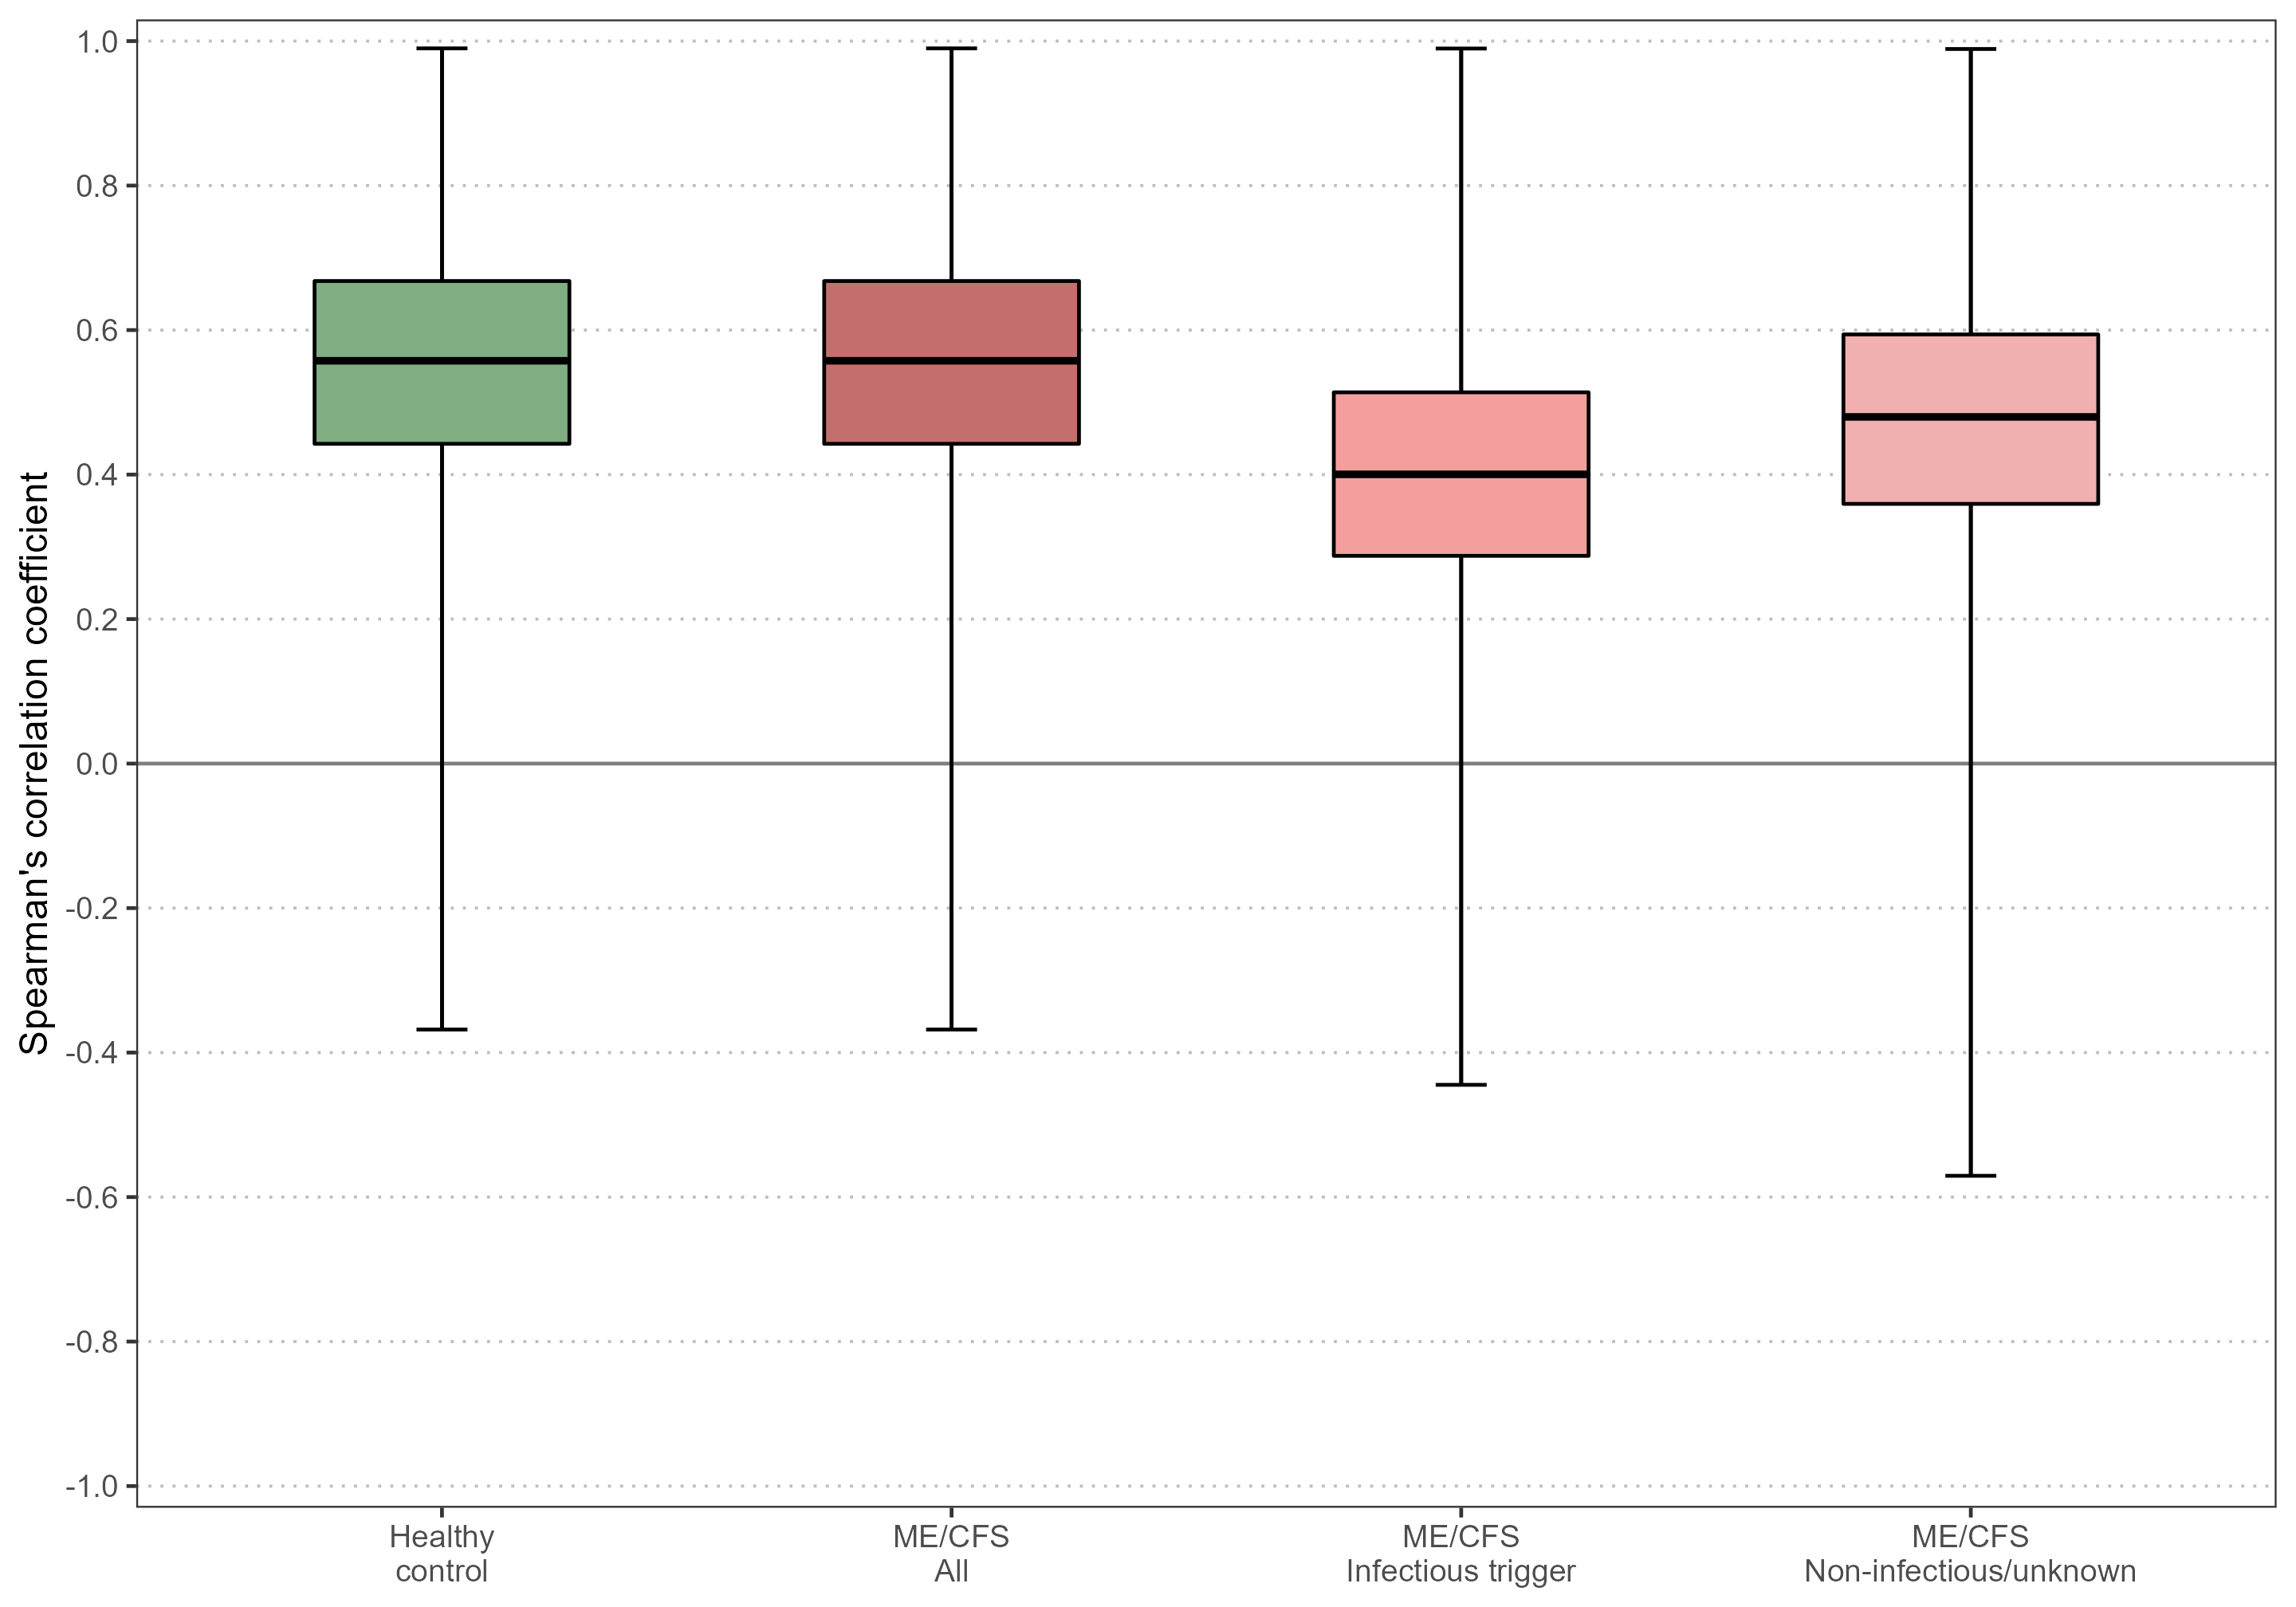
\includegraphics[width=0.85\textwidth]{chapter/2022-revisiting-igg/figures/figa1-ebv-spearmans-correlation.png}
    \caption[Distributions of the Spearman's correlation coefficient between all pairs of EBV-derived antibodies on studied populations]{Distributions of the Spearman's correlation coefficient between all the possible pairs of EBV-derived antibodies in healthy controls, all the ME/CFS patients, ME/CFS patients with an infectious trigger, and ME/CFS patients with a non-infectious or unknown trigger.}
    \label{appendix:figa1-ebv-spearmans-correlation}
\end{figure}
% Supplementary Figure 1
% Supplementary Figure~\ref{appendix:figa1-ebv-spearmans-correlation}